\chapter{Prova de Conceito: \textit{Bot} para Interação Educacional}
\label{cap:prova}

% Usar o graphicspath para buscar figuras no subdiretório figuras
\graphicspath{\currfiledir/figuras/}

Este capítulo apresenta a prova de conceito do \textit{bot} educacional
desenvolvido para este trabalho, detalhando sua implementação técnica e a
metodologia de avaliação experimental proposta. O \textit{dashboard} contém
elementos que são a representação gráfica do \textit{bot}, permitindo ao
professor gerenciar as interações conforme estabelecido no Capítulo
\ref{cap:revisao}.

O Capítulo está organizado da seguinte forma: a Seção \ref{sec:contexto}
contextualiza a interação professor-aluno em ambientes remotos, como
estabelecido no Capítulo \ref{cap:revisao}, e como o \textit{bot} transforma
este paradigma, a Seção \ref{sec:implementacao} detalha os aspectos técnicos da
implementação, incluindo a arquitetura do sistema e as tecnologias utilizadas, a
Seção \ref{sec:funcionalidades} apresenta as funcionalidades implementadas no
\textit{bot} e no \textit{dashboard}, a Seção \ref{sec:metodologia} descreve a
metodologia de avaliação experimental proposta, e finalmente, a Seção
\ref{sec:resultados} apresenta os resultados ilustrativos obtidos na validação
do sistema.

\section{Contexto da Interação Professor-Aluno em Ambientes Remotos}
\label{sec:contexto}

Antes de detalhar os aspectos técnicos da implementação, é importante
contextualizar como ocorre a interação entre professor e alunos em um ambiente
de ensino remoto, particularmente quando se busca aplicar metodologias ativas.

Em aulas remotas tradicionais, observa-se frequentemente um padrão de
comunicação unidirecional, onde o professor transmite o conteúdo enquanto os
alunos assumem postura predominantemente passiva. As interações tendem a ser
limitadas a momentos específicos, como sessões de perguntas ao final da aula, ou
através de canais assíncronos como \textit{e-mails} e fóruns. Este modelo apresenta
barreiras significativas à implementação de metodologias ativas, que dependem de
ciclos rápidos de \textit{feedback} e participação constante dos estudantes.

O \textit{bot} proposto busca transformar este paradigma ao introduzir um
mediador digital que facilita:

\begin{enumerate}
\item \textbf{Trocas síncronas durante a exposição de conteúdo}: Permitindo
reações e dúvidas sem interromper o fluxo da aula
\item \textbf{Anonimato seletivo para alunos}: Reduzindo a inibição de
participação
\item \textbf{Coleta sistemática de dados de interação}: Possibilitando ajustes
em tempo real na condução da aula
\item \textbf{Automação de tarefas repetitivas}: Liberando o professor para
focar em aspectos pedagógicos mais relevantes
\end{enumerate}

Entendemos que estas características são fundamentais para aproximar o ambiente
virtual das dinâmicas interativas observadas em salas de aula presenciais onde
metodologias ativas são aplicadas com sucesso.

\section{Implementação Técnica}
\label{sec:implementacao}

A implementação técnica do sistema educacional segue uma arquitetura dual
composta pelo \textit{bot} Discord e pelo \textit{dashboard} do professor,
conforme conceitualmente apresentado na Seção \ref{subsec:dashboards} do
Capítulo \ref{cap:revisao}. Esta arquitetura garante a separação entre o canal
de comando (exclusivo do professor) e o canal de interação (compartilhado entre
todos os participantes).

\subsection{Arquitetura do \textit{Bot}}

O \textit{bot} foi desenvolvido utilizando a biblioteca Concord em C
(desenvolvida pelo autor deste trabalho). A implementação seguiu uma arquitetura
modular organizada em quatro componentes principais:

\begin{itemize}
\item \textbf{Módulo de Publicação}: Responsável por processar comandos do
professor vindos do \textit{dashboard} e transformá-los em conteúdo formatado
nos canais apropriados do Discord. Este módulo implementa recursos de formatação
para código, imagens e outros materiais didáticos.
\item \textbf{Módulo de Interação}: Gerencia as reações e comandos dos alunos,
incluindo o processamento de \textit{slash commands}, reações com emojis e
mensagens diretas. Este componente implementa o princípio de comunicação
multidirecional discutido na Seção \ref{subsec:principios}.
\item \textbf{Módulo de Análise}: Coleta e processa em tempo real as interações
para gerar métricas de engajamento, barômetros de compreensão e outros
indicadores pedagógicos relevantes. Os resultados são transmitidos ao
\textit{dashboard} do professor para visualização.
\item \textbf{Módulo de Persistência}: Armazena dados estruturados sobre a
sessão para análise posterior, possibilitando a geração de relatórios detalhados
e o acompanhamento longitudinal do progresso dos alunos ao longo de múltiplas
aulas.
\end{itemize}

\begin{figure}[H] \centering
\centering
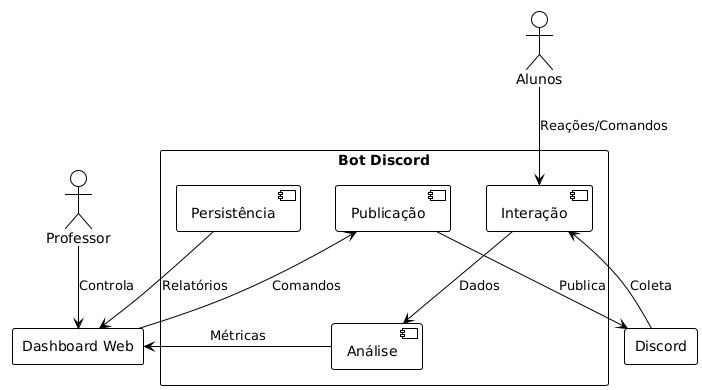
\includegraphics[width=16cm]{arquitetura-bot.png}
\caption{Arquitetura do \textit{bot} educacional, mostrando os principais
módulos e a comunicação com o \textit{dashboard} do professor.}
\label{fig:arquitetura-bot}
\end{figure}

\subsection{Implementação do \textit{Dashboard}}

O \textit{dashboard} do professor foi implementado como uma aplicação web
utilizando tecnologias consolidadas de frontend (Javascript) e backend (Node.js),
comunicando-se com o \textit{bot} através de uma \textit{API REST} segura. Esta
separação arquitetural permite que o professor mantenha uma interface de
controle independente e privada, sem necessidade de interagir diretamente no
\textit{chat} público.

O sistema de comunicação entre \textit{dashboard} e \textit{bot} utiliza um
protocolo de mensagens baseado em WebSockets para garantir atualizações em tempo
real e baixa latência, aspectos cruciais para o controle efetivo da dinâmica da
aula. Esta comunicação bidirecional permite:

\begin{enumerate}
\item Envio de comandos do professor para o \textit{bot} (publicação de
conteúdo, criação de atividades)
\item Transmissão de métricas e alertas do \textit{bot} para o
\textit{dashboard} (nível de engajamento, dúvidas anônimas)
\item Sincronização do estado da aula entre múltiplas sessões de navegador, caso
o professor precise alternar entre dispositivos
\end{enumerate}

\begin{figure}[H] \centering
\centering
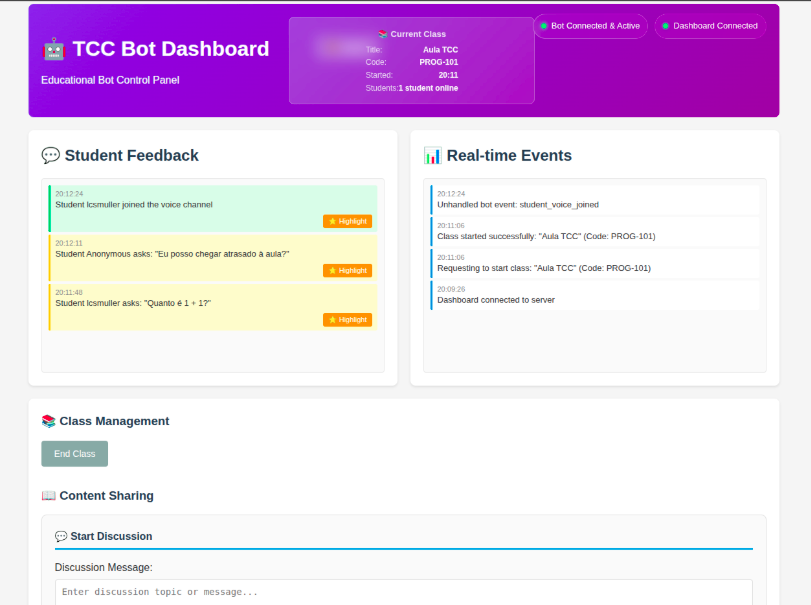
\includegraphics[width=16cm]{dashboard-preview.png}
\caption{Visão geral do \textit{dashboard} do professor, mostrando as principais
funcionalidades e a integração com o \textit{bot} educacional.}
\label{fig:dashboard-preview}
\end{figure}

\subsection{Integração Técnica}

A integração com o Discord foi realizada através das \textit{APIs} fornecidas
pela biblioteca Concord.

A arquitetura implementa os cinco componentes essenciais de um \textit{bot}
educacional descritos na Seção \ref{sec:def-bots}: interface do usuário (canais
do Discord), compreensão de linguagem natural (processamento de comandos),
gerenciador de diálogo (módulo de interação), integração com backend
(\textit{dashboard} e sistemas de persistência) e geração de resposta (módulo de
publicação).

Esta implementação atende diretamente ao objetivo de criar uma prova de conceito
funcional utilizando tecnologias adequadas ao contexto educacional, conforme
estabelecido na Seção \ref{sec:objetivos} do Capítulo \ref{cap:revisao}.

\section{Funcionalidades Implementadas}
\label{sec:funcionalidades}

O sistema desenvolvido consiste em dois componentes principais que trabalham de
forma integrada: (1) o \textit{bot} educacional que interage diretamente com os
alunos no Discord e (2) o \textit{dashboard} exclusivo para o professor que
permite gerenciar essas interações. Esta arquitetura dual implementa o princípio
de "separação de interesses" discutido na Seção \ref{subsec:dashboards} do
Capítulo \ref{cap:revisao}, onde o canal de comando (\textit{dashboard}) é
separado do canal de interação (Discord).

\subsection{Funcionalidades do \textit{Bot} no Discord}
O \textit{bot} no ambiente Discord oferece as seguintes funcionalidades:

\begin{enumerate}
\item \textbf{Mecanismos de \textit{feedback} rápido}: Permite que alunos
utilizem reações para indicar seu nível de compreensão (como "entendi", "tenho
dúvida", "confuso"), criando um barômetro de compreensão em tempo real.
\item \textbf{Canal de dúvidas anônimas}: Os alunos podem enviar dúvidas de
forma privada para o \textit{bot}, que as encaminha ao professor sem identificar
o remetente, reduzindo a inibição.
\item \textbf{Execução de código}: Para disciplinas de programação, o
\textit{bot} permite a execução segura de snippets de código submetidos pelos
alunos, mostrando resultados em tempo real.
\item \textbf{Atividades interativas}: Disponibiliza \textit{quizzes}, enquetes
e desafios temporalizados, coletando e organizando as respostas dos alunos
automaticamente.
\end{enumerate}

\subsection{Funcionalidades do \textit{Dashboard} do Professor}
O \textit{dashboard}, como interface de controle pedagógico, implementa as
seguintes funcionalidades:

\begin{enumerate}
\item \textbf{Sistema de alertas}: Notificações automáticas quando determinados
padrões são detectados, como uma quantidade significativa de alunos indicando
dificuldade.
\item \textbf{Gerenciador de atividades}: Ferramentas para criar, lançar e
monitorar atividades interativas em tempo real.
\item \textbf{Relatórios pós-aula}: Geração de resumos detalhados após a sessão,
incluindo métricas de participação, desempenho e tópicos problemáticos.
\end{enumerate}

Esta integração entre \textit{dashboard} e \textit{bot} cria um sistema coeso
que permite ao professor manter o controle pedagógico da aula enquanto facilita
interações dinâmicas com os alunos. O professor pode, por exemplo, identificar
rapidamente conceitos que geraram confusão através do \textit{dashboard} e
adaptar sua abordagem ou enviar explicações adicionais através do \textit{bot},
sem interromper o fluxo da aula.

A Figura \ref{fig:dashboard-bot} (Capítulo \ref{cap:revisao}) ilustra esta
relação integrada, onde o \textit{dashboard} atua como interface de comando
exclusiva do professor, enquanto o \textit{bot} serve como ponto de contato e
interação para todos os participantes.

\section{Metodologia de Avaliação}
\label{sec:metodologia}

A metodologia de avaliação para o \textit{bot} educacional consiste em uma
abordagem experimental com participantes reais assumindo os papéis de professor
e alunos em um ambiente de sala de aula simulado, conforme delineado na Seção
\ref{sec:objetivos} do Capítulo \ref{cap:revisao}. Esta abordagem permite
avaliar a eficácia da ferramenta em condições próximas ao uso real, combinando
métricas quantitativas e qualitativas.

\subsection{Ambiente e Participantes}
\label{subsec:ambiente}

O experimento foi conduzido em ambiente controlado com:

\begin{itemize}
\item Participantes de diversas áreas e níveis de formação atuando como
professores (controlando o \textit{dashboard}) e como alunos (interagindo via
Discord)
\item Sessões simuladas de aulas remotas reproduzindo cenários pedagógicos
típicos
\end{itemize}

\subsection{Coleta de Dados}
\label{subsec:coleta}

Os dados são coletados através de três mecanismos principais:

\begin{enumerate}
\item \textbf{Questionários}: Aplicados a professores e alunos para medir
percepções sobre o uso do \textit{bot} e o \textit{dashboard}. O questionário
completo e suas respostas detalhadas estão documentados no Apêndice
\ref{cap:dados-experimentais}.
\item \textbf{Registros automáticos (\textit{logs})}: Dados quantitativos sobre
frequência e tipos de interações realizadas
\item \textbf{Entrevistas}: Conduzidas com participantes para obter insights
qualitativos
\end{enumerate}

\subsection{Métricas de Avaliação}
\label{subsec:metricas}

As seguintes métricas são utilizadas para avaliar a eficácia da solução:

\begin{table}[htb]
\centering
\caption{Métricas para avaliação da eficácia do \textit{bot}}
\label{tab:metricas}
\begin{tabular}{|p{3cm}|p{9cm}|}
\hline
\textbf{Categoria} & \textbf{Métricas} \\
\hline
\textbf{Engajamento} & Número de interações por aluno, distribuição temporal das
interações, diversidade de tipos de interação \\
\hline
\textbf{Impacto pedagógico} & Mudanças na condução da aula, percepção de
compreensão do conteúdo, tempo dedicado a esclarecimentos \\
\hline
\textbf{Usabilidade} & Facilidade de uso, problemas técnicos, curva de
aprendizado \\
\hline
\textbf{Metodologias ativas} & Viabilidade de implementação, comparação com
experiências presenciais \\
\hline
\end{tabular}
\end{table}

\section{Resultados Ilustrativos}
\label{sec:resultados}

O experimento foi conduzido com 10 participantes que atuaram tanto no papel de
professor quanto no papel de aluno, permitindo uma avaliação abrangente da
ferramenta sob ambas as perspectivas. Os dados foram coletados através de
questionários aplicados após a participação no experimento, abordando aspectos
de usabilidade, eficácia pedagógica e percepção geral da ferramenta. Os dados
completos da avaliação, incluindo gráficos detalhados e comentários na íntegra,
estão disponíveis no Apêndice \ref{cap:dados-experimentais}.

\subsection{Dados Quantitativos}
\label{subsec:dados-quant}

A análise quantitativa dos questionários revelou resultados promissores em
múltiplas dimensões avaliadas. As respostas foram coletadas em escala Likert de
1 a 5, onde 1 representa "muito insatisfatório" e 5 representa "muito
satisfatório".

\subsubsection{Usabilidade e Facilidade de Uso}

Quanto à facilidade de uso do \textit{bot}, 80\% dos participantes atribuíram
notas 4 ou 5, com média de 4,3. Este resultado indica que a interface do
\textit{bot} foi considerada intuitiva pela maioria dos usuários, apesar de
alguns comentários sugerirem melhorias na forma de interação com comandos.

Para o \textit{dashboard} do professor, entre os participantes que o utilizaram,
a avaliação foi ainda mais positiva, com média de 4,5 e todos os respondentes
atribuindo notas 4 ou 5, demonstrando que a interface de controle pedagógico
atendeu adequadamente às expectativas.

\subsubsection{Eficácia Pedagógica}

No quesito "ajuda na compreensão do conteúdo", o \textit{bot} obteve média de
4,1, com 70\% dos participantes atribuindo notas 4 ou 5. Este resultado sugere
que a ferramenta efetivamente contribuiu para o processo de aprendizagem,
alinhando-se com os objetivos pedagógicos estabelecidos.

Quanto ao impacto na interatividade das aulas, os resultados foram
excepcionalmente positivos: 90\% dos participantes concordaram que o \textit{bot}
tornou a aula mais interativa (notas 4 ou 5), com média de 4,7. Este foi o
aspecto mais bem avaliado, confirmando a eficácia da ferramenta em promover
metodologias ativas.

\subsubsection{Redução de Carga e Facilitação da Comunicação}

Sobre a redução da carga de trabalho do professor, a média foi de 3,8, indicando
uma percepção moderadamente positiva. Já na facilitação da comunicação, a média
foi de 4,7, com 90\% dos participantes atribuindo notas máximas, demonstrando
que o \textit{bot} efetivamente melhorou os canais de comunicação entre
professor e alunos.

\subsubsection{Aceitação e Adoção}

Um indicador importante de sucesso foi a alta disposição para adoção da
ferramenta: 90\% dos participantes manifestaram desejo de que o \textit{bot}
fosse utilizado em mais aulas (notas 4 ou 5), com média de 4,6. Este resultado
sugere forte aceitação e potencial de adoção real da tecnologia.

\subsubsection{Funcionalidades Mais Utilizadas}

As funcionalidades mais populares foram:
\begin{itemize}
\item Reações: utilizadas por 70\% dos participantes
\item Dúvidas anônimas: utilizadas por 60\% dos participantes  
\item Execução de código: utilizadas por 60\% dos participantes
\item \textit{Quizzes}: utilizados por 70\% dos participantes
\end{itemize}

\subsection{Análise Qualitativa}
\label{subsec:analise-qual}

A análise dos comentários textuais forneceu \textit{insights} valiosos sobre a
experiência dos usuários e direcionamentos para melhorias futuras.

\subsubsection{Aspectos Mais Valorizados}

Os participantes destacaram consistentemente o valor do anonimato como principal
benefício da ferramenta. Comentários como "Poder comentar em anônimo e não ser
necessário responder em áudio" e "Possibilidade do anonimato" foram recorrentes,
confirmando que esta funcionalidade efetivamente reduz barreiras de participação
em ambientes remotos.

A interatividade foi outro aspecto amplamente elogiado, com destaque para a
capacidade de "tornar o chat um canal mais viável para interagir com o
professor" e "poder responder digitando e não precisar falar". Estes comentários
evidenciam que o \textit{bot} conseguiu criar alternativas eficazes aos modelos
tradicionais de interação em aulas remotas.

O \textit{dashboard} do professor recebeu elogios específicos por permitir
"resumir o chat dos alunos ao final da aula" e "conseguir criar enquetes de
maneira bem intuitiva", demonstrando que a separação entre canal de comando e
canal de interação foi bem-sucedida.

\subsubsection{Limitações e Sugestões de Melhoria}

A principal crítica recorrente refere-se à interface de comandos. Múltiplos
participantes sugeriram substituir comandos de texto por botões interativos:
"Uma maneira mais fácil de responder coisas sem ter que usar comandos, por
exemplo, botão" e "Responder de maneira mais fácil, sem ter que usar comandos,
utilizando um botão".

Outras sugestões incluem:
\begin{enumerate}
\item Melhorar a experiência de resposta inline (evitar modais para comandos
simples)
\item Implementar notificações mais proeminentes para o professor
\item Adicionar controles para moderação de conteúdo anônimo
\item Desenvolver \textit{exports} em formatos mais amigáveis que JSON
\end{enumerate}

\subsubsection{Impacto na Dinâmica Educacional}

Os comentários revelaram que o \textit{bot} efetivamente alterou a dinâmica das
aulas remotas. Um participante observou que a ferramenta "torna o chat um canal
mais viável para interagir com o professor, geralmente o professor esquece o
chat e foca somente no canal de voz", indicando que o sistema conseguiu abordar
uma limitação real do ensino remoto.

A redução do isolamento também foi mencionada, com participantes relatando que
a ferramenta "reduziu sensação de isolamento", sugerindo que as funcionalidades
interativas contribuíram para um senso maior de comunidade virtual.

\subsubsection{Considerações sobre Adoção Real}

Os comentários indicam que, apesar das limitações de interface identificadas, os
participantes reconheceram o valor pedagógico da ferramenta. A disposição para
uso em contextos reais foi expressa tanto por aspectos técnicos ("consegue
visualizar melhor as interações via chat nas aulas") quanto pedagógicos
("permite que você faça perguntas sem que seus colegas julguem você").

Esta análise qualitativa confirma que o \textit{bot} atendeu aos objetivos
principais de facilitar metodologias ativas em ambientes remotos, embora
melhorias na experiência do usuário possam amplificar significativamente sua
eficácia e adoção.
